\begin{figure}
     \centering
     \begin{subfigure}{0.4\textwidth}
         \centering
         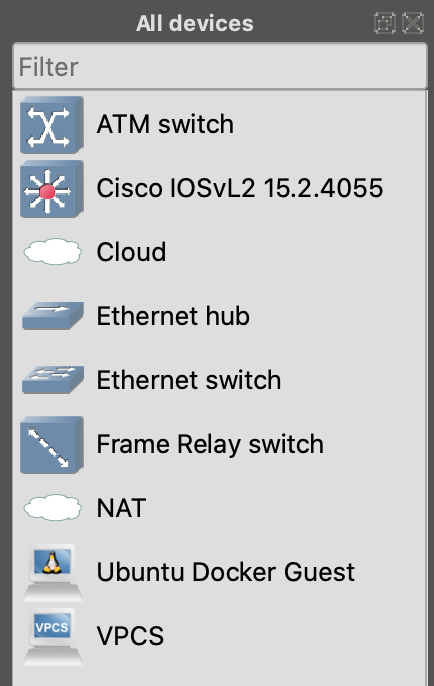
\includegraphics[width=\textwidth]{gns3-appliances-dock}
         \caption{The appliances dock}
         \label{fig:gns3-appliances-dock}
     \end{subfigure}
     \hfill
     \begin{subfigure}{0.5\textwidth}
         \centering
         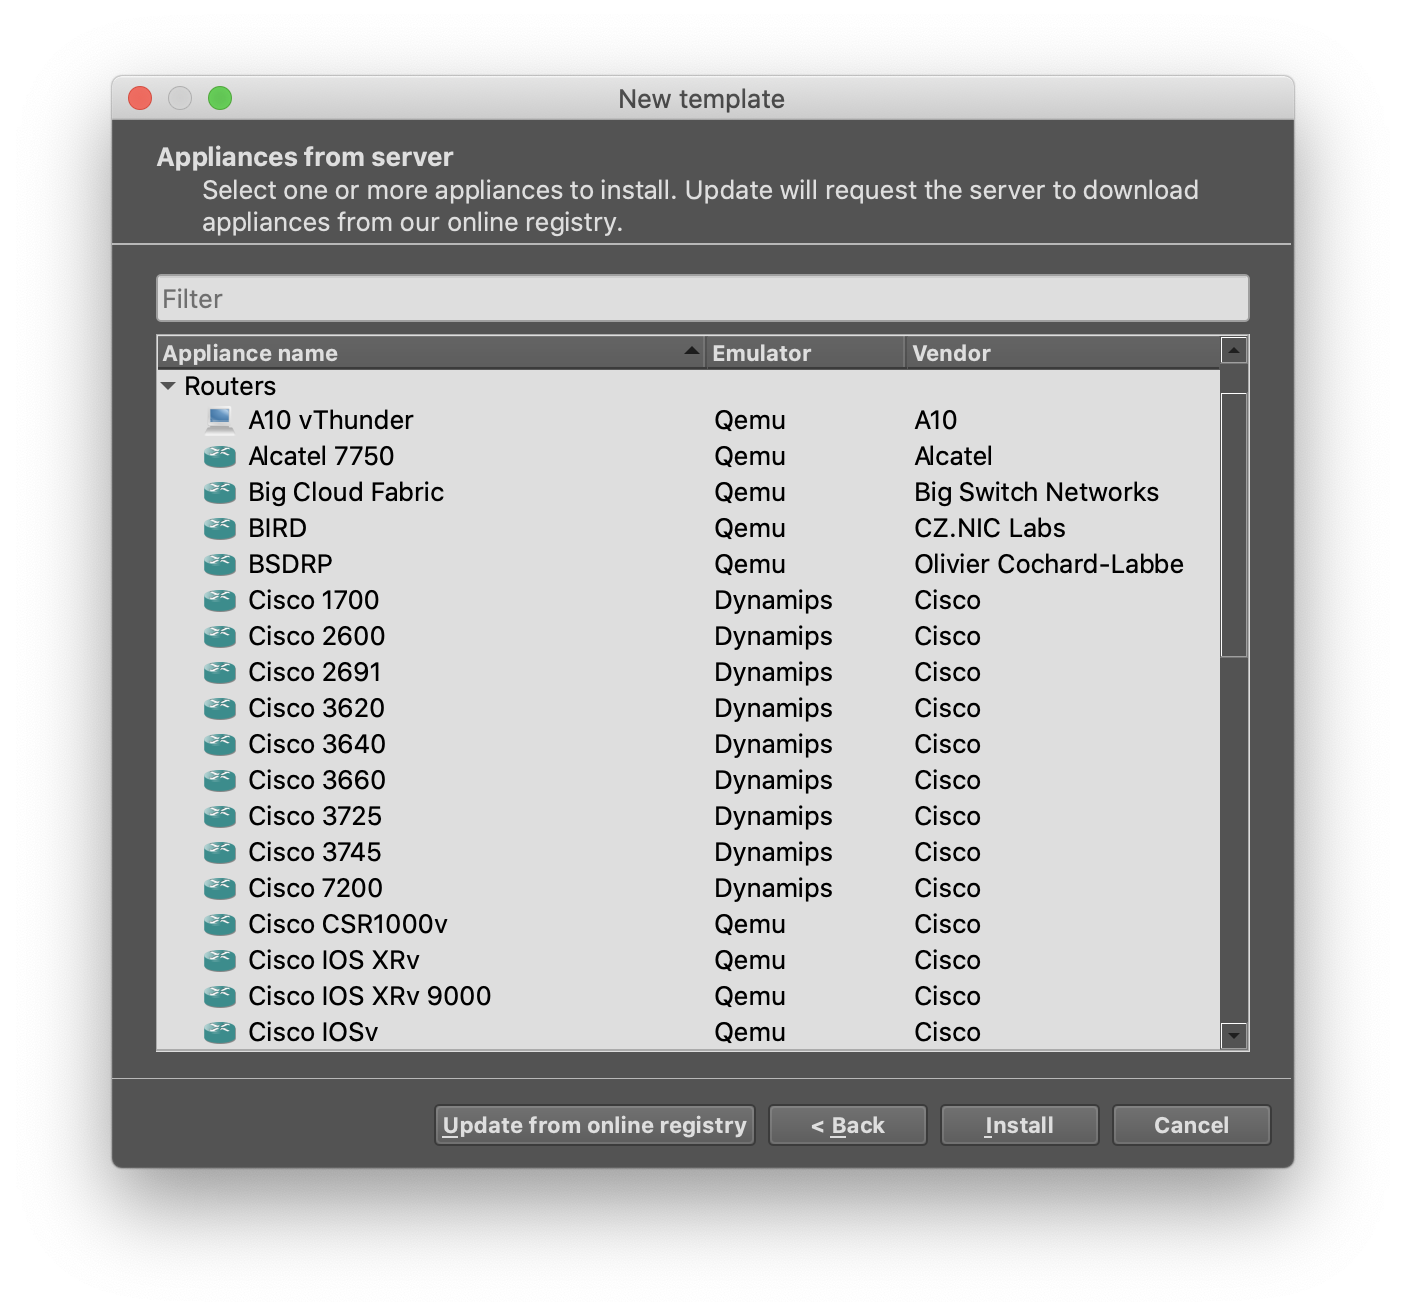
\includegraphics[width=\textwidth]{gns3-appliances-from-server-routers}
         \caption{Some available router templates}
         \label{fig:gns3-appliances-from-server-routers}
     \end{subfigure}
    \caption{Using and installing appliances in the GNS3 GUI}
    \label{fig:gns3-appliances}
\end{figure}

% For reference, below a way to put figures side-by-side without considering them subfigures

% \begin{figure}
% \centering
% \begin{minipage}{.4\textwidth}
%   \centering
%   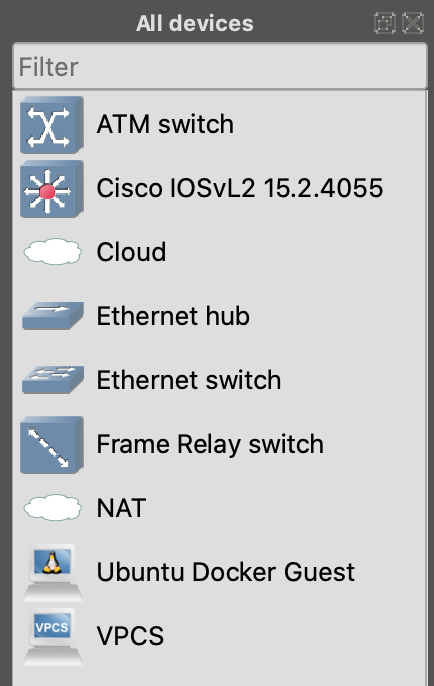
\includegraphics[width=.8\linewidth]{gns3-appliances-dock}
%   \captionof{figure}{The appliances dock}
%   \label{fig:gns3-appliances-dock}
% \end{minipage}%
% \begin{minipage}{.6\textwidth}
%   \centering
%   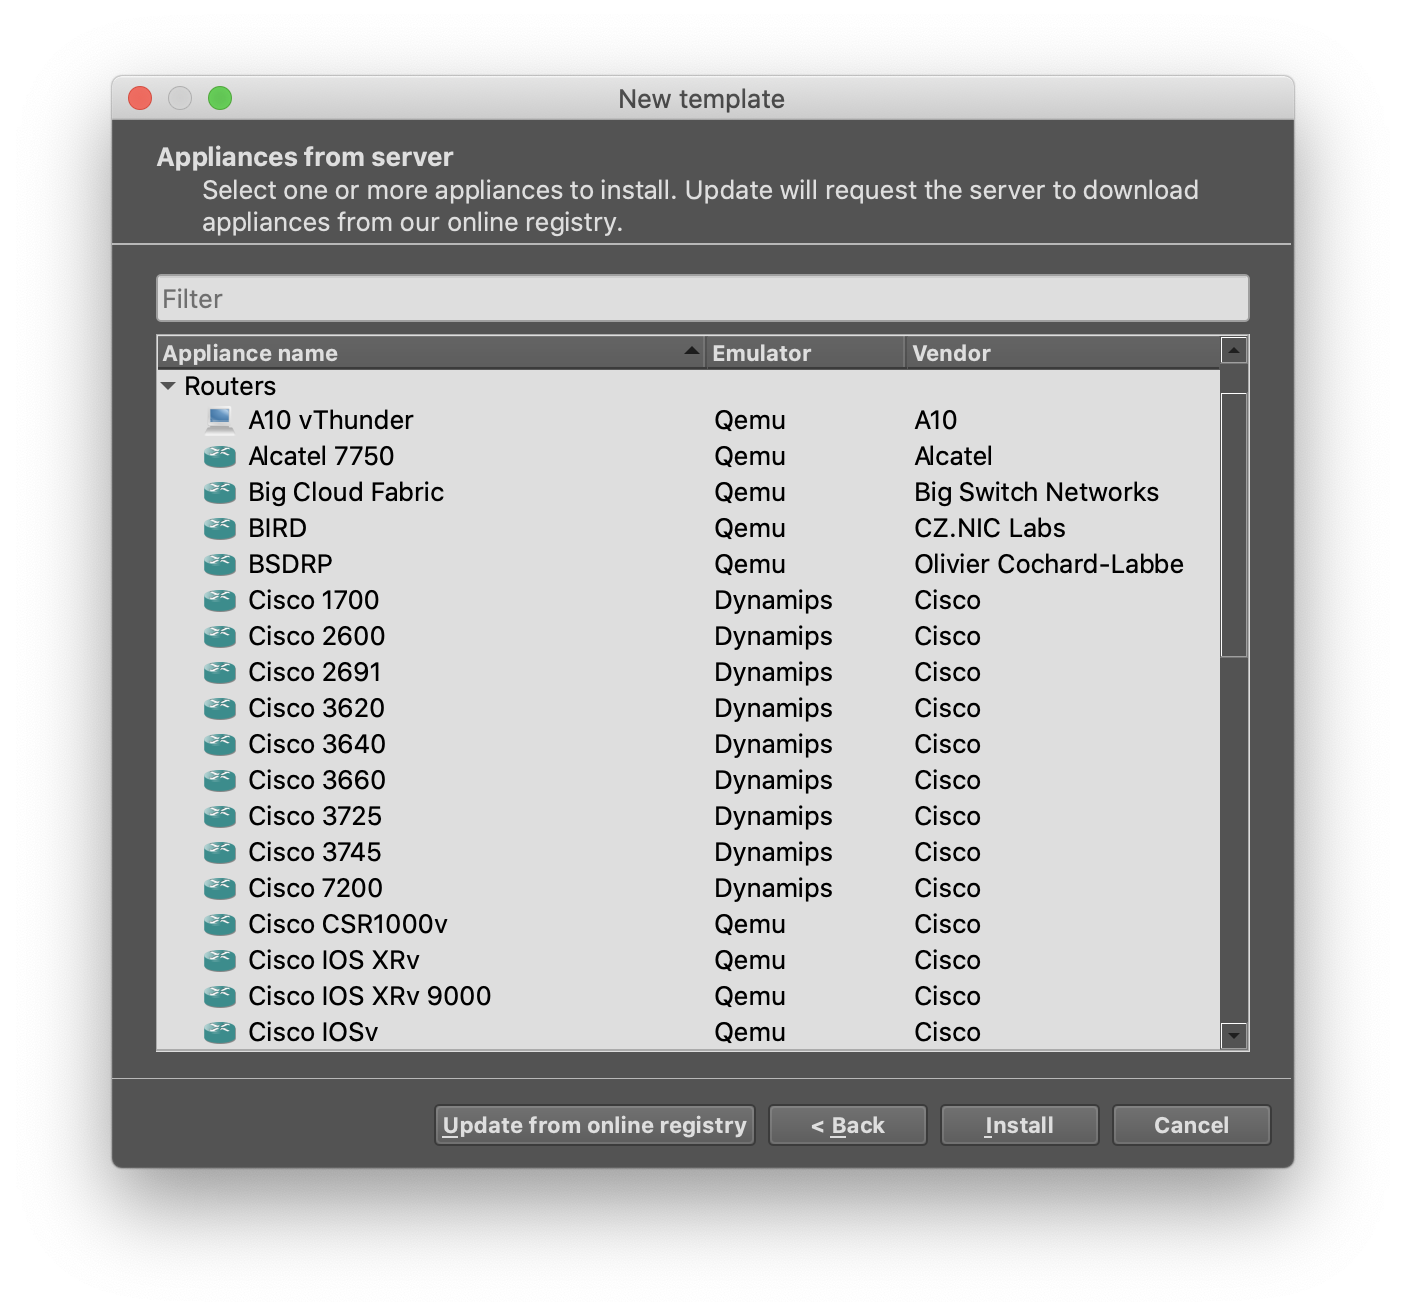
\includegraphics[width=.95\linewidth]{gns3-appliances-from-server-routers}
%   \captionof{figure}{Some available router templates}
%   \label{fig:gns3-appliances-from-server-routers}
% \end{minipage}
% \end{figure}
